\documentclass[12pt]{article}
\usepackage[left=1cm, right=1cm, top=2cm,bottom=1.5cm]{geometry} 

\usepackage[parfill]{parskip}
\usepackage[utf8]{inputenc}
\usepackage[T2A]{fontenc}
\usepackage[russian]{babel}
\usepackage{enumitem}
\usepackage[normalem]{ulem}
\usepackage{amsfonts, amsmath, amsthm, amssymb, mathtools,xcolor}
\usepackage{blkarray}

\usepackage{tabularx}
\usepackage{hhline}

\usepackage{accents}
\usepackage{fancyhdr}
\pagestyle{fancy}
\renewcommand{\headrulewidth}{1.5pt}
\renewcommand{\footrulewidth}{1pt}

\usepackage{graphicx}
\usepackage[figurename=Рис.]{caption}
\usepackage{subcaption}
\usepackage{float}

%%Наименование папки откуда забирать изображения
\graphicspath{ {./images/} }

%%Изменение формата для ввода доказательства
\renewcommand{\proofname}{$\square$  \nopunct}
\renewcommand\qedsymbol{$\blacksquare$}

%%Изменение отступа на таблицах
\addto\captionsrussian{%
	\renewcommand{\proofname}{$\square$ \nopunct}%
}
%% Римские цифры
\newcommand{\RN}[1]{%
	\textup{\uppercase\expandafter{\romannumeral#1}}%
}

%% Для удобства записи
\newcommand{\MR}{\mathbb{R}}
\newcommand{\MC}{\mathbb{C}}
\newcommand{\MQ}{\mathbb{Q}}
\newcommand{\MN}{\mathbb{N}}
\newcommand{\MZ}{\mathbb{Z}}
\newcommand{\MTB}{\mathbb{T}}
\newcommand{\MTI}{\mathbb{I}}
\newcommand{\MI}{\mathrm{I}}
\newcommand{\MCI}{\mathcal{I}}
\newcommand{\MJ}{\mathrm{J}}
\newcommand{\MH}{\mathrm{H}}
\newcommand{\MT}{\mathrm{T}}
\newcommand{\MU}{\mathcal{U}}
\newcommand{\MV}{\mathcal{V}}
\newcommand{\MB}{\mathcal{B}}
\newcommand{\MF}{\mathcal{F}}
\newcommand{\MW}{\mathcal{W}}
\newcommand{\ML}{\mathcal{L}}
\newcommand{\MP}{\mathcal{P}}
\newcommand{\VN}{\varnothing}
\newcommand{\VE}{\varepsilon}

\theoremstyle{definition}
\newtheorem{defn}{Опр:}
\newtheorem{rem}{Rm:}
\newtheorem{prop}{Утв.}
\newtheorem{exrc}{Упр.}
\newtheorem{problem}{Задача}
\newtheorem{lemma}{Лемма}
\newtheorem{theorem}{Теорема}
\newtheorem{corollary}{Следствие}

\newenvironment{cusdefn}[1]
{\renewcommand\thedefn{#1}\defn}
{\enddefn}

\DeclareRobustCommand{\divby}{%
	\mathrel{\text{\vbox{\baselineskip.65ex\lineskiplimit0pt\hbox{.}\hbox{.}\hbox{.}}}}%
}
%Короткий минус
\DeclareMathSymbol{\SMN}{\mathbin}{AMSa}{"39}
%Длинная шапка
\newcommand{\overbar}[1]{\mkern 1.5mu\overline{\mkern-1.5mu#1\mkern-1.5mu}\mkern 1.5mu}
%Функция знака
\DeclareMathOperator{\sgn}{sgn}

%Функция ранга
\DeclareMathOperator{\rk}{\text{rk}}
\DeclareMathOperator{\diam}{\text{diam}}


%Обозначение константы
\DeclareMathOperator{\const}{\text{const}}

\DeclareMathOperator{\codim}{\text{codim}}

\DeclareMathOperator*{\dsum}{\displaystyle\sum}
\newcommand{\ddsum}[2]{\displaystyle\sum\limits_{#1}^{#2}}

%Интеграл в большом формате
\DeclareMathOperator{\dint}{\displaystyle\int}
\newcommand{\ddint}[2]{\displaystyle\int\limits_{#1}^{#2}}
\newcommand{\ssum}[1]{\displaystyle \sum\limits_{n=1}^{\infty}{#1}_n}

\newcommand{\smallerrel}[1]{\mathrel{\mathpalette\smallerrelaux{#1}}}
\newcommand{\smallerrelaux}[2]{\raisebox{.1ex}{\scalebox{.75}{$#1#2$}}}

\newcommand{\smallin}{\smallerrel{\in}}
\newcommand{\smallnotin}{\smallerrel{\notin}}

\newcommand*{\medcap}{\mathbin{\scalebox{1.25}{\ensuremath{\cap}}}}%
\newcommand*{\medcup}{\mathbin{\scalebox{1.25}{\ensuremath{\cup}}}}%

\makeatletter
\newcommand{\vast}{\bBigg@{3.5}}
\newcommand{\Vast}{\bBigg@{5}}
\makeatother

%Промежуточное значение для sup\inf, поскольку они имеют разную высоту
\newcommand{\newsup}{\mathop{\smash{\mathrm{sup}}}}
\newcommand{\newinf}{\mathop{\mathrm{inf}\vphantom{\mathrm{sup}}}}

%Скалярное произведение
\newcommand{\inner}[2]{\left\langle #1, #2 \right\rangle }
\newcommand{\linsp}[1]{\left\langle #1 \right\rangle }
\newcommand{\linmer}[2]{\left\langle #1 \vert #2\right\rangle }

%Подпись символов снизу
\newcommand{\ubar}[1]{\underaccent{\bar}{#1}}

%% Шапка для букв сверху
\newcommand{\wte}[1]{\widetilde{#1}}
\newcommand{\wht}[1]{\widehat{#1}}

%%Трансформация Фурье
\newcommand{\fourt}[1]{\mathcal{F}\left(#1\right)}
\newcommand{\ifourt}[1]{\mathcal{F}^{-1}\left(#1\right)}

%%Символ вектора
\newcommand{\vecm}[1]{\overrightarrow{#1\,}}

%%Пространстов матриц
\newcommand{\mat}[2]{\operatorname{Mat}_{#1\times #2}}


%%Взятие в скобки, модули и норму
\newcommand{\parfit}[1]{\left( #1 \right)}
\newcommand{\modfit}[1]{\left| #1 \right|}
\newcommand{\sqparfit}[1]{\left\{ #1 \right\}}
\newcommand{\normfit}[1]{\left\| #1 \right\|}

%%Функция для обозначения равномерной сходимости по множеству
\newcommand{\uconv}[1]{\overset{#1}{\rightrightarrows}}
\newcommand{\uconvm}[2]{\overset{#1}{\underset{#2}{\rightrightarrows}}}


%%Функция для обозначения нижнего и верхнего интегралов
\def\upint{\mathchoice%
	{\mkern13mu\overline{\vphantom{\intop}\mkern7mu}\mkern-20mu}%
	{\mkern7mu\overline{\vphantom{\intop}\mkern7mu}\mkern-14mu}%
	{\mkern7mu\overline{\vphantom{\intop}\mkern7mu}\mkern-14mu}%
	{\mkern7mu\overline{\vphantom{\intop}\mkern7mu}\mkern-14mu}%
	\int}
\def\lowint{\mkern3mu\underline{\vphantom{\intop}\mkern7mu}\mkern-10mu\int}

%%След матрицы
\DeclareMathOperator*{\tr}{tr}

\makeatletter
\renewcommand*\env@matrix[1][*\c@MaxMatrixCols c]{%
	\hskip -\arraycolsep
	\let\@ifnextchar\new@ifnextchar
	\array{#1}}
\makeatother


%% Переопределение функции хи, чтобы выглядела более приятно
\makeatletter
\@ifdefinable\@latex@chi{\let\@latex@chi\chi}
\renewcommand*\chi{{\@latex@chi\smash[t]{\mathstrut}}} % want only bottom half of \mathstrut
\makeatletter

\begin{document}
\lhead{Математический анализ - \RN{2}}
\chead{Косухин О.Н.}
\rhead{Семинар - 1}

\section*{Неопределенный интеграл}

Пусть $F(x)$ определена на промежутке $\inner{a}{b}$, где  $\langle \in \{\, (, [ \, \}, \, \rangle \in \{\, ),] \, \}$ и $a,b$ могут принимать бесконечные значения: $\pm \infty$.

\begin{defn}
	$F(x)$ называется \uwave{первообразной} для $f(x)$ (на $\inner{a}{b}$), если $F'(x) = f(x), \, \forall x \in \inner{a}{b}$.
\end{defn}
Первообразная не обязательна существует, но для многих она есть.

\begin{theorem}
	Пусть $F_1(x)$ и $F_2(x)$ - две первообразные для $f$ на $<a,b>$, тогда: 
	$$
		F_1(x) - F_2(x) = \const, \, \forall x \in \inner{a}{b}
	$$ 
\end{theorem}
\begin{proof}
	Рассмотрим разность как функцию: $F(x) = F_1(x) - F_2(x) \Rightarrow F'(x) = f(x) - f(x) = 0$. Рассмотрим разность этой функции в разных точках: $F(x_2) - F(x_1)$, где $x_1, x_2 \in \inner{a}{b}$. Пусть $x_2 > x_1$, тогда по теореме Лагранжа:
	$$
		F(x_2) - F(x_1) = F'(c)(x_2 - x_1), \, c \in (x_1, x_2) \Rightarrow F'(x)= 0 \Rightarrow F(x_2) - F(x_1) = 0 \Rightarrow F(x) = \const
	$$
\end{proof}

Пусть $M = \{F(x) \colon F\text{ - первообразная для } f \text{ на }\inner{a}{b}\}$, тогда оно имеет следующий вид:
$$
	M = \{F_0(x) + C \colon C \in \MR\} = \ddint{}{}f(x)dx 
$$
\begin{defn}
	Множество $M$ всех первообразных функции $f$ называется \uwave{неопределенным интегралом} $f$.
\end{defn}
Стилизованное обозначение интеграла идёт от буквы $S$ (square). В таком выражении есть большой недостаток: нигде не фигурирует промежуток $\inner{a}{b}$ и он как бы подразумевается из контекста.

\section*{Таблица неопределенных интегралов}

\subsection*{Степенные функции}
$1)$ $(x^n)' = nx^{n-1} \Rightarrow \ddint{}{}nx^{n-1}dx = x^n + C \Rightarrow \ddint{}{}x^{n-1}dx = \dfrac{x^n}{n} + C$.

При $n = 1$ мы получаем следующий интеграл: 
$$
	\ddint{}{}1{\cdot}dx = x + C
$$

При $p \in \MR, \, x \in (0,+\infty)$ мы получим: 
$$
	\ddint{}{}x^pdx = \dfrac{x^{p+1}}{p+1} + C
$$ 
При $p \in \MN$ равенство будет верно $\forall x \in \MR$.
\begin{rem}
	Отметим, что здесь обязательно $p \neq -1$.
\end{rem}

Можно заметить, что у нас множество недоговорок и при решении задач будем опускать конкретные детали на каком промежутке мы отыскали ту или иную первообразную. Рассмотрим также один исключительный случай, когда $p = -1$. 

$2)$ $(\ln{(x)})' = \dfrac{1}{x} \Rightarrow x > 0, \, \ddint{}{}\dfrac{1}{x}dx = \ln{(x)} + C$. $(\ln{(-x)})' = \dfrac{-1}{-x} = \dfrac{1}{x} \Rightarrow x<0, \, \ddint{}{}\dfrac{1}{x}dx = \ln{(x)} + C$.

Часто пишут: 
$$
	\ddint{}{}\dfrac{1}{x}dx = \ln{|x|} + C, \, x \neq 0
$$ 
В этой записи собраны две записи выше для первого промежутка и для второго. Но неверно утверждать, что множество всех первообразных для $\frac{1}{x}$ на объединении $(-\infty, 0) \cup (0,+\infty)$ будет тем, что обозначено выше. Дело в том, что можно взять $\ln{(x)}$ и двигать её вверх/вниз, прибавляя свою константу $C_1$. Тоже самое можно делать для $\ln{(-x)}$, прибавляя свою константу $C_2$.

\begin{figure}[H]
	\centering
	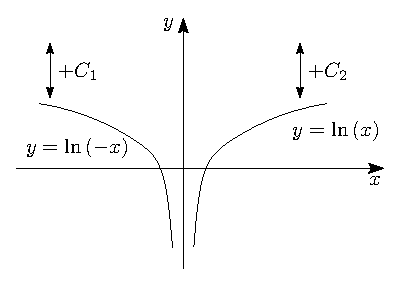
\includegraphics[width=0.4\textwidth]{MA2S1_1.eps}
	\caption{Множество $y = \ln{|x|} + C$.}
	\label{1_1}
\end{figure}
Но делать такие сдвиги мы можем только независимо. Мы же все рассуждения делаем только для промежутков и запись выше лишь означает, что содержит в себе два равенства для сокращения:
$$
	\ddint{}{}\dfrac{1}{x}dx = 
	\begin{cases}
		\ln{(x)} + C_1, & x > 0 \\
		\ln{(-x)} + C_2, & x < 0
	\end{cases}
$$

\subsection*{Показательные функции}
$3)$ $\ddint{}{}e^x dx = e^x + C, \, x \in \MR$.

$4)$ $\ddint{}{}a^xdx = \dfrac{a^x}{\ln{a}} + C, \, x \in \MR$.

\subsection*{Тригонометрические функции}
$5)$ $\ddint{}{}\sin{x}dx = -\cos{x} + C, \, x\in \MR$. 

$6)$ $\ddint{}{}\cos{x}dx = \sin{x} + C, \, x \in \MR$.
\begin{rem}
	Когда пишут неопределенный интеграл, то обычно опускают скобочки подразумевающие что интеграл это множество, а не одна какая-то функция.
\end{rem}

$7)$ $\ddint{}{}\dfrac{1}{\cos^2{x}}dx = \ddint{}{}(1 + \tg^2{x})dx = \tg{x} + C$.

И опять, равенство выше подразумевается для тех промежутков, где $\frac{1}{\cos^2{x}}$ определена: то есть для любого промежутка, который лёг между точками $\frac{(2k-1)\pi}{2}$ и $\frac{(2k +1)\pi}{2}$:
$$
	x \in \inner{a}{b} \subset \left(\dfrac{(2k-1)\pi}{2}, \dfrac{(2k+1)\pi}{2}\right), \, k \in \MZ
$$

$8)$ $\ddint{}{}\dfrac{1}{\sin^2{x}}dx = \ddint{}{}(1 + \ctg^2{x})dx = -\ctg{x} + C$.

И опять же, равенство подразумевается для промежутков, где $\frac{1}{\sin^2{x}}$ определена.

\subsection*{Обратные тригонометрические функции}
$9)$ $(\arcsin{x})' = \dfrac{1}{\sqrt{1 - x^2}} \Rightarrow  \ddint{}{}\dfrac{1}{\sqrt{1 - x^2}}dx = \arcsin{x} + C, \, x \in (-1,1)$.

$10)$ $(\arccos{x})' = -\dfrac{1}{\sqrt{1 - x^2}} \Rightarrow  \ddint{}{}\dfrac{1}{\sqrt{1 - x^2}}dx = -\arccos{x} + C, \, x \in (-1,1)$.

Отсюда можем утверждать, что множества первообразных выше равны:
$$
	\{\arcsin{x} + C \colon C \in \MR\} = \{-\arccos{x} + C \colon C \in \MR\}
$$
Но сами представители этих множеств не равны между собой. По теореме выше, эти два представления отличаются на константу и действительно:
$$
	\arcsin{x} + \arccos{x} \equiv \dfrac{\pi}{2}
$$

$11)$ $\ddint{}{}\dfrac{1}{1 + x^2}dx =  \left[
\begin{array}{c}
	\arctg{x} + C \\[5pt]
	-\arcctg{x} + C
\end{array}
\right., \, x \in \MR$.

Аналогично предыдущему случаю:
$$
	\arctg{x} + \arcctg{x} \equiv \dfrac{\pi}{2}
$$

\subsection*{Гиперболические функции}
$$
	\sh{x} = \sinh{x} = \dfrac{e^x - e^{-x}}{2}, \, \ch{x} = \cosh{x} = \dfrac{e^x + e^{-x}}{2}, \, \th{x} = \dfrac{\sh{x}}{\ch{x}} 
$$
$12)$ $(\sh{x})' = \ch{x} \Rightarrow \ddint{}{}\sh{x}dx = \ch{x} + C$.

$13)$ $(\ch{x})' = \sh{x} \Rightarrow \ddint{}{}\ch{x}dx = \sh{x} + C$.

$14)$ $(\th{x})' = \dfrac{\ch^2{x} - \sh^2{x}}{\ch^2{x}} = \dfrac{1}{\ch^2{x}} \Rightarrow \ddint{}{}\dfrac{1}{\ch^2{x}}dx = \th{x} + C$.

$15)$ $(\cth{x})' = \dfrac{\sh^2{x} - \ch^2{x}}{\sh^2{x}} = -\dfrac{1}{\sh^2{x}} \Rightarrow \ddint{}{}\dfrac{1}{\sh^2{x}}dx = -\cth{x} + C$.

\subsection*{Обратные гиперболические функции}
Рассмотрим гиперболические функции и попробуем понять, как устроены обратные гиперболические функции. Для этого нужно понимать, а где это вообще можно сделать.
\begin{figure}[H]
	\centering
	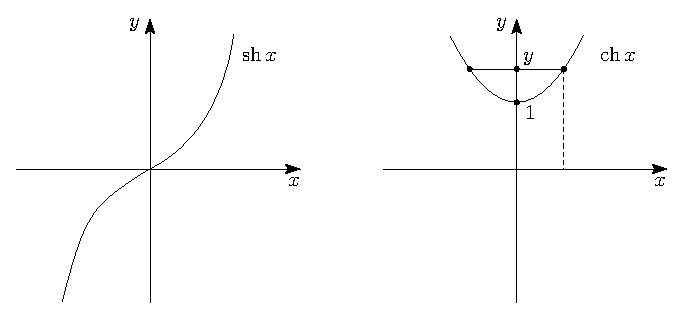
\includegraphics[width=0.6\textwidth]{MA2S1_2.eps}
	\caption{Гиперболические функции.}
	\label{1_2}
\end{figure}
Видим, что обратная функция для гиперболического синуса: $x = \sh^{-1}{(y)}$ существует везде и называется \uwave{ариасинус}. Обратная функция для гиперболического косинуса: $x = \ch^{-1}{(y)}$ существует только при $y \geq 1$ и при этом надо выбирать какой-то конкретный $x$, как правило это: $x > 0$, называется обратная функция \uwave{ариакосинус}. Решим уравнения:
$$
	y = \dfrac{e^x - e^{-x}}{2} \Rightarrow t = e^{x} \neq 0 \Rightarrow t - \dfrac{1}{t} = 2y \Rightarrow t^2 -2yt -1 = 0 \Rightarrow \dfrac{D}{4} = y^2 + 1, \, t = y \pm\sqrt{y^2 + 1}
$$
Заметим, что $\sqrt{y^2 + 1} > |y|$ и если взять отрицательную часть , то $t < 0 \Rightarrow t = y + \sqrt{y^2 + 1}$. Тогда:
$$
	e^x = y + \sqrt{y^2 + 1} \Rightarrow x = \ln{\left(y + \sqrt{y^2 + 1}\right)}
$$
это ариасинус. Такое выражение называют ``длинным логарифмом''. Для косинуса похожая ситуация:
$$
	t = e^x \Rightarrow t +\dfrac{1}{t} = 2y \Rightarrow t^2 - 2yt + 1 = 0 \Rightarrow \dfrac{D}{4} = y^2 - 1 \Rightarrow t = y \pm \sqrt{y^2 - 1} 
$$
Если договорились на $x \geq 0$, то берём корень: $t = y + \sqrt{y^2 -1}$. Ариакосинус будет равен:
$$
	e^x =t = y + \sqrt{y^2 -1} \Rightarrow x = \ln{\left(y + \sqrt{y^2 - 1}\right)}
$$

$16)$ $\left(\ln{(y + \sqrt{y^2 + p})}\right)' = \dfrac{1 + \frac{y}{\sqrt{y^2 + p}}}{y + \sqrt{y^2 + p}} = \dfrac{1}{\sqrt{y^2 + p}} \Rightarrow \ddint{}{}\dfrac{dx}{\sqrt{x^2 + p}} = \ln{\left|x + \sqrt{x^2 + p}\right|} + C$.

Заметим, что выражение выше верно при $y^2 + p > 0$.

\subsection*{Способы приведения интегралов к табличным}
\begin{enumerate}[label=\arabic*)]
	\item \uline{\textbf{Замена переменной}}: всегда можно менять обозначение у буквы:
	$$
		\ddint{}{}f(x)dx = F(x) + C \Leftrightarrow \ddint{}{}f(u)du = F(u) + C
	$$
	\item \uline{\textbf{Линейность}}: по аналогии со свойством линейности для производных:
	$$
		F'(x) = f(x), \, G'(x) = g(x) \Rightarrow  (A{\cdot}F(x) + B{\cdot}G(x))' = Af(x) +  Bg(x) \Rightarrow
	$$
	$$
		\Rightarrow \ddint{}{}Af(x) + Bg(x)dx = A\ddint{}{}f(x)dx + B\ddint{}{}g(x) dx
	$$
	\item \uline{\textbf{Подстановка линейной функции}}: подставим вместо аргумента линейную функцию:
	$$
		F'(x) = f(x) \Rightarrow (F(at + b))' = af(at + b) \Rightarrow \ddint{}{}af(at + b)dt = F(at + b) + C \Rightarrow
	$$
	$$
		\Rightarrow \ddint{}{}f(at + b)dt = \dfrac{1}{a}F(at + b) + C
	$$
\end{enumerate}

\begin{problem}(\textbf{Д1633})
	$$\ddint{}{}\dfrac{x+1}{\sqrt{x}}dx$$
\end{problem}
\begin{proof}
	Поскольку деление на корень из $x$, то промежуток подразумевается $(0, +\infty)$. Запишем $x = \sqrt{x}\sqrt{x}$:
	$$
		\ddint{}{}\dfrac{x+1}{\sqrt{x}}dx = \ddint{}{}\sqrt{x} + \dfrac{1}{\sqrt{x}}dx = \ddint{}{}\sqrt{x}dx + \ddint{}{}\dfrac{1}{\sqrt{x}}dx = \ddint{}{}x^{\frac{1}{2}}dx + \ddint{}{}x^{-\frac{1}{2}}dx = \dfrac{2x^{\frac{3}{2}}}{3} + 2x^{\frac{1}{2}} + C
	$$
\end{proof}
\newpage
\begin{problem}(\textbf{Д1642})
	$$\ddint{}{}\dfrac{\sqrt{1 + x^2} + \sqrt{1 - x^2}}{\sqrt{1 - x^4}}dx$$
\end{problem}
\begin{proof}
	Поскольку деление на корень из $1 -x^4$, то промежуток подразумевается $(-1, 1)$:
	$$
		\sqrt{1 - x^4} = \sqrt{1 - x^2}{\cdot}\sqrt{1 + x^2} \Rightarrow 
	$$
	$$	
		\Rightarrow \ddint{}{}\dfrac{\sqrt{1 + x^2} + \sqrt{1 - x^2}}{\sqrt{1 - x^4}}dx = \ddint{}{}\dfrac{1}{\sqrt{1-x^2}}dx + \ddint{}{}\dfrac{1}{\sqrt{1 + x^2}}dx = \arcsin{x} + \ln(x + \sqrt{1 + x^2}) + C
	$$
\end{proof}

\begin{problem}(\textbf{Д1648})
	$$\ddint{}{}\sqrt{1-\sin{2x}}dx, \, 0 \leq  x \leq \pi$$
\end{problem}
\begin{proof}
	$$
		\ddint{}{}\sqrt{1-\sin{2x}}dx = \ddint{}{}\sqrt{\sin^2{x} + \cos^2{x} - 2\sin{x}\cos{x}}dx = \ddint{}{}\sqrt{(\cos{x} - \sin{x})^2}dx = \ddint{}{}|\cos{x} - \sin{x}|dx
	$$
	На разных промежутках модуль раскрывается по-разному $\Rightarrow$ нам будет важен промежуток.
	\begin{figure}[H]
		\centering
		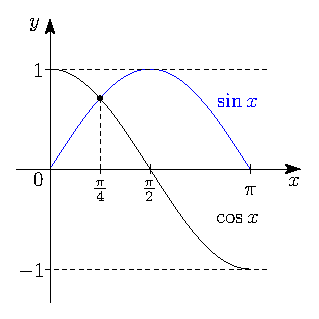
\includegraphics[width=0.3\textwidth]{MA2S1_3.eps}
		\caption{$\sin{x}, \, \cos{x}$ на отрезке $[0,\pi]$.}
		\label{1_3}
	\end{figure}
	$$
		|\cos{x} - \sin{x}| = 
		\begin{cases}
			\cos{x} - \sin{x}, & x \in\left[0,\frac{\pi}{4}\right]\\
			\sin{x} - \cos{x}, & x\in \left[\frac{\pi}{4},\pi\right]
		\end{cases} \Rightarrow \ddint{}{}|\cos{x} - \sin{x}|dx = 
	\begin{cases}
		\sin{x} + \cos{x} + C_1, & x \in\left[0,\frac{\pi}{4}\right]\\
		-\cos{x} - \sin{x} + C_2, & x\in \left[\frac{\pi}{4},\pi\right]
	\end{cases}
	$$
	При $x = \frac{\pi}{4}$ мы получим $\sqrt{2} + C_1 = -\sqrt{2} + C_2 \Rightarrow C_2 = 2\sqrt{2} + C_1$. То есть только одна константа может быть свободной. Итого:
	$$
		F(x) = 	
		\begin{cases}
			\sin{x} + \cos{x} + C, & x \in\left[0,\frac{\pi}{4}\right]\\
			-\cos{x} - \sin{x} + 2\sqrt{2} + C, & x\in \left[\frac{\pi}{4},\pi\right]
		\end{cases}
	$$
	Будет ли эта функция дифференцируема в точке $\frac{\pi}{4}$? По следствию $1$ лекции $25$ семестра $1$ у дифференцируемой функции могут быть только разрывы $\RN{2}$-го рода. Поскольку $F(x)$ - непрерывна в этой точке, то если у этой функции есть левые/правые пределы, то они должны быть равны: 
	$$
		\lim\limits_{x \to \frac{\pi}{4}+}F'(x) = \lim\limits_{x \to \frac{\pi}{4}-}F'(x) \Rightarrow \exists \,  F'\left(\frac{\pi}{4}\right) = f\left(\frac{\pi}{4}\right)
	$$
	$$
		\cos{x} - \sin{x} \xrightarrow[x\to \frac{\pi}{4}+]{} 0 ,\, \sin{x} - \cos{x} \xrightarrow[x\to \frac{\pi}{4}-]{} 0 \Rightarrow \lim\limits_{x \to \frac{\pi}{4}+}F'(x) = \lim\limits_{x \to \frac{\pi}{4}-}F'(x) \Rightarrow F'\left(\frac{\pi}{4}\right) = f\left(\frac{\pi}{4}\right)
	$$
	Таким образом, мы корректно нашли первообразную, поскольку на ``склейке'' функций, наша функция интегрируема.
\end{proof}


\subsection*{Обобщенная первообразная}
Рассмотрим функцию $y = |x|$. Её производная выглядит как $\sgn{x}$, если мы доопределим эту функцию в нуле нулём. Для неё не существует первообразной в окрестности точки $0$. Иначе, пределфункции слева и справа: $F'(0+)= 1$ и $F'(0-) = -1 \Rightarrow$ функция была бы недифференцируемой в $0$. 

\begin{defn}
	Пусть есть $\inner{a}{b}$ и функция $f(x)$ на нем. $F(x)$ называется \uwave{обобщенной первообразной}, если:
	\begin{enumerate}[label=\arabic*)]
		\item $F(x) \in C(\inner{a}{b})$;
		\item $\exists$ конечное множество точек $\mathrm{E} = \{x_1,\dotsc, x_n\} \subset \inner{a}{b} = \MI$ такое, что:
		$$
			\forall x \in \MI \setminus \mathrm{E}, \, F'(x) = f(x)
		$$
	\end{enumerate}
\end{defn}
То есть мы не отказываемся от условий непрерывности, но при этом этой функции разрешается некоторое количество нарушений: в точках $x_1, \dotsc, x_n$ либо производная может не существовать, либо она может не совпадать с $f(x)$. Когда найти первообразную будет невозможно, мы будем искать обобщенную первообразную.
\begin{rem}
	Иногда разрешают счетное число точек.
\end{rem}
\begin{rem}
	Если функция - первообразная, то она - обобщенная первообразная. Обратно не верно.
\end{rem}

\textbf{Пример}: Примером обобщенной первообразной может быть $y = |x|$ на $\MR$ для функции $f(x) = \sgn{x}$ с точкой $x = 0$  из свойства $2)$. Для обобщенных первообразных также работает теорема $1$:
$$
	\ddint{}{}\sgn{x}dx = |x| + C
$$

\begin{problem}
	$$
		\ddint{}{}\dfrac{1}{x^2 - 1}dx 
	$$
\end{problem}
\begin{proof}
	$$
		\ddint{}{}\dfrac{1}{x^2 - 1}dx= \ddint{}{}\dfrac{1}{(x-1)(x+1)}dx = \ddint{}{}\dfrac{A}{x-1}dx + \ddint{}{}\dfrac{B}{x +1}dx
	$$
	Данный метод решения называется \uwave{методом неопределенных коэффициентов}:
	$$
		\dfrac{Ax + A + Bx -B}{x^2 -1} = \dfrac{1}{x^2 -1} \Rightarrow A + B = 0 \wedge A - B = 1 \Rightarrow 2A = 1 \Rightarrow A = \dfrac{1}{2}, \, B = -\dfrac{1}{2} \Rightarrow
	$$
	$$
		\Rightarrow \ddint{}{}\dfrac{A}{x-1}dx + \ddint{}{}\dfrac{B}{x +1}dx = \dfrac{1}{2}\ddint{}{}\dfrac{1}{x-1}dx - \dfrac{1}{2}\ddint{}{}\dfrac{1}{x+1}dx =
	$$
	$$
		= \dfrac{1}{2}\ln{|x-1|} - \dfrac{1}{2}\ln{|x+1|} + C = \dfrac{1}{2}\ln{\left|\dfrac{x-1}{x+1}\right|} + C
	$$
\end{proof}

\textbf{ДЗ}: $1635$, $1643$, $1646$ (вспомнить сумму кубов), $1650$, $1656$, $1659$, $1667$, $1672$.

\textbf{ДЗ}: найти $\th^{-1}(y)$, $\cth^{-1}(y)$ и посчитать их производные. 
\end{document}